%! TEX root = main.tex

본 연구는 영지식 증명을 사전 정의된 범위에 적용한 최초의 검색 시스템이므로, 직접적으로 비교할 수 있는 동일한 기능의 선행 연구가 존재하지 않는다. 따라서 본 장에서는 시스템의 실효성을 입증하기 위해 벤치마크 실험과 데이터의 원문을 저장하여 실시간으로 증명을 생성하는 baseline 모델을 구현하고 처리 시간과 용량 부담을 비교 측정하는 실험을 진행한다. 이로써 본 연구가 제시하는 '사전 생성된 증명에 대한 검색 시스템'의 효율성과 의의, 그리고 한계(trade-off) 등을 종합적으로 분석한다.

\subsection{실험 설계}

\subsubsection{마이크로 벤치마크}
우선 본 연구에서 사용하는 두가지 영지식 증명: 범위 증명과 소유권 증명에 대한 각각의 처리 시간을 측정한다. 한 속성 데이터에 대해 범위 증명을 생성하는데 소요되는 평균 시간과 다수의 데이터에 대한 소유권 증명을 생성하는데 소요되는 평균 시간을 측정한다. 범위 증명의 경우, 시스템에 등록된 DI의 수에 따라 회로의 크기가 달라지므로 이를 128, 256, 512, 1024로 지수적으로 증가시키며 시간을 측정한다. 소유권 증명의 경우, 처리하고자 하는 서브 쿼리의 수가 고정되어 있지 않으므로 최소 2개부터 시작하여 최대 5개까지 선형적으로 늘렸을 때 추가 소요되는 시간을 확인한다. 이렇게 시스템 성능의 핵심 요소인 영지식 증명의 처리 시간을 측정하여, 대규모 시스템에 적용하였을 시, 어느 정도까지의 부하를 감당해야 하는지를 예측할 수 있다.

\bigskip

또한 범위 증명과 소유권 증명에 대해 증명 데이터의 평균 크기도 함께 측정한다. Groth16 프로토콜의 특성상, 회로의 구조나 규모에 관계없이 증명 데이터의 크기는 항상 일정할 것으로 예상되며, 이를 확인할 것이다. 또한 데이터 원문은 단순 정수로, 4~8바이트 정도로 크기가 작은데 비해, 증명 데이터 바이너리는 크기가 상대적으로 크기 때문에 어느 정도의 용량 부하가 추가되는지 확인할 필요가 있다. 사전에 생성하여 저장하는 범위 증명 데이터의 크기는 시스템의 스토리지 부하에 영향을 끼치며, 실시간으로 생성되는 소유권 증명 데이터의 크기는 네트워크 부하에 영향을 끼칠 것이다.

\bigskip

마지막으로 실제 시스템에서 다중 쿼리를 처리하는데 소요된 시간을 상세히 측정할 것이다. 빈 응답이 없도록 구성한 다중 쿼리 100개를 한 세트로 하여, 서브 쿼리의 숫자를 2에서 5로 늘려가며 응답 시간을 측정한다. 이를 통해 실제 검색 시스템에서 사용자가 기다려야 하는 시간과, 전체 응답 시간 중 실시간 영지식 증명이 차지하는 비율을 확인할 것이다. 이를 통해 소유권 증명을 위한 실시간 증명의 트레이드 오프가 충분히 수용할 만한 수준이라는 것을 증명할 것이다.

\subsubsection{설계 방식 비교 실험}
본 연구가 제안하는 시스템의 가장 큰 특징은 사전 정의된 범위(pre-defined range)를 기반으로 증명 데이터를 발급 시점에 미리 생성하고, 검색 시점에 이를 조회하는 방식이다. 이로써 데이터 원문은 보유하지 않으면서 그것의 존재를 효율적으로 확인하는 것이 가능하다. 하지만 현실의 대부분의 검색 시스템은 데이터 원문을 보관하고 쿼리에 따라 원문의 속성을 직접 조회하는 방식으로 동작한다. 이같이 데이터 원문을 제 3자인 검색 서버가 보유하는 것은 시스템의 보안을 크게 훼손하는 일이나, 대부분의 경우, 이처럼 고객의 동의 하에 각종 개인정보를 위탁 관리하고 있다. 따라서 baseline 모델을 다음과 같이 정의하고, 본 연구가 제안하는 '사전에 생성된 증명 검색' 방식의 성능을 비교하였다.

\begin{itemize}
  \item 실시간 증명(on-the-fly ZKP): 데이터 원문을 데이터베이스에 저장한 후, 쿼리의 범위를 만족하는 튜플들을 조회하여 해당 튜플에 대한 범위 증명을 실시간(on-the-fly)으로 생성하여 반환하는 시스템.
  \item 측정 지표: 평균 쿼리 응답 시간. 정해진 100개의 쿼리에 대해 결과를 반환하기 까지의 시간을 측정하여 그에 대한 평균을 계산.
  \item 기대 결과: baseline은 조회되는 데이터의 수(페이지 크기)에 따라 수 초 이상이 소요될 수 있지만 제안 시스템은 밀리초(ms) 단위로 즉시 응답함을 보여 실용성을 입증.
\end{itemize}

또한 baseline 모델을 설계할 때, 원문을 암호화 하였을 때와, 하지 않았을 경우를 별도로 비교한다. 이는 성능을 우선하여 구현한 경우와 보안을 우선하여 구현한 경우를 제안된 모델과 함께 비교하기 위함이다. 원문을 암호화 할 경우, 쿼리 처리 과정에서 복호화 과정이 추가되며, 이는 곧 추가적인 성능 하락이 있을 수 있음을 암시한다. 암호 알고리즘은 AES-CTR을 채택한다. AES 알고리즘은 블록 기반 암호화 알고리즘으로, 블록 스킴(CBC, GCM 등)을 선택해야 하는데, 이 경우 CTR 스킴을 선택하였다. 이는 암호화 하는 데이터가 최대 64비트의 정수(수치형 데이터이므로)인데, CBC나 GCM과 같은 대중적인 블록 스킴을 사용하면 64비트의 용량 제한을 넘어서기 때문이다. 데이터 원문을 문자열의 형태로 저장하는 방법도 있지만 이는 불필요한 형변환 과정을 발생시키므로 처리 속도에 영향을 미친다. 반면 CTR 스킴은 스트림 암호화 스킴으로, 원문과 암호문의 크기가 동일하다. 따라서 실험의 환경에서 최적의 속도를 기대할 수 있다.

\bigskip

실험은 100만개($N = 10^6$) 데이터 셋을 임의로 생성하여 진행한다. 먼저 정해진 1000명의 DP 정보와 30개 속성 정보를 기반으로 100만 개의 데이터를 무작위로 생성하여 base 데이터베이스를 구성한다. 그리고 이를 기반으로 다시 서로 다른 DI 숫자(128, 256, 512, 1024)를 가진 각각의 환경에 대응하는 최종 데이터베이스를 생성한다. 이를 통해 발급자 정보만 다를 뿐, 데이터의 분포는 완전히 동일한 4개의 테스트 셋이 구성된다. 이 base 데이터베이스는 baseline 모델 뿐만 아니라, 제안 모델에서도 동일하게 활용되어, 총 12개의 동일한 분포를 지닌 테스트 셋이 만들어진다. 이로써 서로 다른 테스트 셋들이 DI 정보를 제외, 완벽히 동일한 데이터를 기반으로 구성되도록 한다.

\bigskip

실험은 다음 두 파라미터를 변경해가며 진행한다. 

\begin{itemize}
    \item \textbf{DI 수:} 시스템에 등록된 발급자(DI)의 수에 따라 범위 증명의 영지식 회로의 규모가 달라진다. 따라서 DI수를 달리 했을 때, 어느 정도로 부하가 증가하는지 측정하고 확장성을 판단한다. 실험에선 128, 256, 512, 1024의 DI를 사용한다.
    \item \textbf{페이지 크기:} 모든 검색 시스템은 처리 시간과 네트워크 부하 등의 이유로 기본적으로 페이징 시스템을 차용한다. 즉, 한번에 반환하는 페이지의 크기에 따라 응답시간도 변화할 수 밖에 없다. 따라서 페이지 크기를 점진적으로 늘렸을 때 어느 정도의 처리 지연이 발생하는지 측정하고 확장성을 판단한다. 기본 페이지 크기를 30으로 설정하였고 이를 60, 90, 120으로 늘리며 처리 시간을 비교 측정한다.
\end{itemize}

마지막으로 실험 환경에서 baseline 모델과 제안 모델이 사용한 데이터베이스와 각종 파일들의 용량을 비교할 것이다. baseline 모델은 정수형의 원문 데이터를 데이터베이스의 일부로 보관하지만 본 연구의 시스템은 원문 대신 증명 데이터를 별도의 바이너리 파일로 보관하기 때문에 어느정도 스토리지 부담이 증가할 수 밖에 없다. 따라서 실험 환경의 100만개 데이터가 만들어내는 스토리지 부하를 서로 다른 DI의 수에 따라 각각 측정하여 비교한다.

\subsubsection{위협 모델 시뮬레이션 및 확장 보안에 대한 고찰}

본 제안 시스템은 소유권 증명 쿼리 처리의 실시간성을 확보하기 위해, 검색 서버(SS) 내부에 민감 데이터인 OWNERSHIP 맵핑 테이블을 유지하는 반신뢰(Semi-honest) 위협 모델을 기본으로 설계되었다. 그렇기에 검색 서버가 외부 공격자나 악의적인 관리자에 의해 완전히 장악되어 OWNERSHIP 테이블을 포함한 모든 데이터베이스가 유출되는 최악의 시나리오를 가정할 경우, 프라이버시 침해 위협이 발생할 수 있다. 따라서 공격자의 입장에서 OWNERSHIP 데이터베이스를 장악했을 경우를 가정하여 취득한 데이터를 분석하고 시각화하는 시뮬레이션을 진행한다. 나아가 이러한 위협을 완화하기 위해 고려 가능한 전략을 함께 간략히 소개한다.

\subsection{실험 환경}

본 실험은 macOS를 구동하며, 애플 M4 프로세서, 16GB 통합 메모리, 256GB SSD 저장 공간을 지닌 Apple Mac Mini 환경에서 진행하였다. 실험에 사용된 모든 시스템 컴포넌트는 Go 언어(v1.25.1)로 작성되어 동일한 로컬 머신 상에서 구동되었으며, 측정된 시간 지표들은 네트워크 통신 지연을 배제한 순수 시스템 연산 시간을 기준으로 한다. 영지식 증명 프레임워크로는 gnark(v0.14.0)를 사용하였고, 회로 최적화를 위해 BN254 타원곡선과 MiMC 해시, EdDSA 서명 알고리즘을 적용하였다. 데이터베이스는 SQLite(v1.6.0)를, ORM 라이브러리로는 gorm(v1.31.1)을 사용하였다.

\bigskip

실험에 사용한 데이터는 총 1,000,000건($10^6$) 규모로, 모두 임의로 생성하여 앞서 언급한 base 데이터베이스를 구성하였다. 이는 본 시스템에서 다루는 데이터의 형태가 단일 수치로, 다른 데이터와 상호 관계성이 전무하므로 문제가 없다는 판단에 기반하였다. 생성된 수치 값들은 각 항목의 특성을 반영하여 주어진 범위 내에서 균등 분포(Uniform Distribution)를 가지도록 난수로 생성되었다. 데이터 속성 정보의 경우 실제 의료 데이터 거래 시나리오를 재현하기 위해 서울아산병원 건강정보 \cite{asan2014}를 참고하여 '당화혈색소', '공복혈당' 등 30개의 검진 데이터 항목을 수기로 작성하여 적용하였다. DP 정보는 1000개의 비대칭키 쌍을 생성하여 사용하였고 DI 정보는 각각 128, 256, 512, 1024개의 비대칭키 쌍을 생성하여 사용하였다.

\subsection{실험 결과}

\subsubsection{마이크로 벤치마크}

\begin{table}[h]
    \footnotesize
    \centering
    \begin{tabular}{p{3cm}|c|c|c|c}
        \hline
        DI Count & 128 & 256 & 512 & 1024 \\
        \hline
        Proof Gen Time(ms) & 75 & 80 & 83 & 86 \\
        Proof Size(Bytes) & 164 & 164 & 164 & 164 \\
        \hline
    \end{tabular}
    \caption{range proof benchmark}
\end{table}

\begin{table}[h]
    \footnotesize
    \centering
    \begin{tabular}{p{3cm}|c|c|c|c}
        \hline
        Sub-query Count& 2 & 3 & 4 & 5 \\
        \hline
        Proof Gen Time(ms) & 10 & 11 & 12 & 16 \\
        Proof Size(Bytes) & 164 & 164 & 164 & 164 \\
        \hline
    \end{tabular}
    \caption{ownership proof benchmark}
\end{table}

마이크로 벤치마크 실험에선 범위 증명과 소유권 증명에 대한 증명 생성 시간과 크기을 각각 측정하였다. 이를 통해 다음 세가지 사실을 입증할 수 있었다.

\bigskip

첫째, 범위 증명의 경우 시스템에 등록된 데이터 발급자(DI)의 수가 128개에서 1024개로 8배 증가함에 따라 증명 생성 시간은 75ms에서 86ms로 단 11ms(약 15\%) 증가하는 데 그쳤다. 이는 영지식 회로 내부에서 수행되는 발급자 공개키에 대한 머클 증명 연산이 $O(\log{N})$의 시간 복잡도를 가지기 때문이다. 즉, 발급 기관의 수가 대규모로 확장되더라도 개별 증명 생성 시간에 미치는 영향이 매우 미미함을 입증한다. 이를 통해 본 시스템의 확장성은 시스템에 등록되는 발급자의 수에 큰 영향을 받지 않음을 예측할 수 있다.

\bigskip

둘째, 다중 쿼리 처리를 위한 소유권 증명의 경우, 서브 쿼리의 개수가 2개에서 5개로 늘어날 때, 증명 생성 시간은 9ms에서 16ms로 소폭 증가하였다. 서브 쿼리의 개수가 증가할수록 개별 증명들의 식별자를 해싱하여 prf\_hash를 구하는 연산량이 늘어나지만, 최대 5개의 복합 조건을 처리할 때조차 절대적인 증명 생성 시간이 16ms로 매우 가볍다. 이 결과는 본 연구의 4.6.1절에서 제안한 소유권 증명에 대한 '실시간 일괄 생성' 최적화의 타당성을 뒷받침한다. 즉, 다중 쿼리에 대한 소유권 증명을 검색 서버(SS)가 쿼리 시점에 실시간으로 생성하더라도, 서버 연산에 미치는 부담이 극히 적어 높은 실시간성을 확보할 수 있음을 보여준다.

\bigskip

셋째, 파라미터나 회로의 구조에 관계 없이 모든 경우의 증명 데이터 크기가 일정하다. 이는 zk-SNARK의 특장점으로, 증명 대상의 속성에 관계없이 늘 일정한 크기의 증명 데이터가 보장된다. 이는 시스템을 확장했을 때 요구되는 스토리지 오버헤드를 쉽게 예측할 수 있게 해준다. 실제로 실험을 위해 생성한 $10^6$개 데이터에 대해 생성된 증명 데이터는 약 630 메가바이트로 측정되었다. 이는 검증의 편의성을 위해 공개 파라미터를 증명 데이터와 함께 저장하였기에, 나온 수치이다. 공개 파라미터를 제외하고 순수히 증명 데이터만 저장한다면 이를 약 164 메가바이트로 줄일 수 있다. 또한 페이지 크기가 30일 때 다중 쿼리에 대한 응답으로 반환되는 소유권 증명 크기의 총합은 164 $\times$ 30 = 4,920 바이트, 약 4.9 킬로바이트에 해당한다. 이는 일반적인 저해상도 이미지 한장, 혹은 그 이하에 해당하는 수준이기에 네트워크 부담을 크게 증가시키지 않는다. 이와 같이 zk-SNARK(Groth16)의 증명 데이터는 충분히 크기가 작으며 또한 고정되어있기에 대량의 데이터에 대해서도 용량 부담을 일으키지 않으며, 확장에 대한 리소스 예측을 용이하게 한다.

\bigskip

\begin{table}[h]
    \centering
    \footnotesize
    \begin{tabular}{l|c|c|c|c}
        \hline
        Sub-query Count & 2 & 3 & 4 & 5 \\
        \hline
        Overall & 3,711 & 5,340 & 7,156 & 9,019 \\
        DB Fetch & 3,253 & 4,878 & 6,696 & 8,556 \\
        Proof Gen & 454 & 458 & 457 & 459 \\
        \hline
    \end{tabular}
    \caption{average query response time(ms) for different sizes of composite query(128 DI, page size 30)}
    \label{tab:placeholder}
\end{table}

다중 쿼리에 대한 벤치마크 결과는 위와 같았다. 100개의 다중 쿼리에 대한 전체 응답 시간과 데이터베이스 조회 시간, 증명 생성 시간을 별도로 기록하였다. 서브 쿼리의 갯수에 상관없이, 모든 환경에서 소유권 증명 데이터의 생성 시간은 동일한 수준(약 457ms)이었다. 이는 소유권 증명이 단순한 해시 비교를 수행하는 회로로 구성되기 때문에 파라미터의 크기에 거의 영향을 받지 않으며, 충분히 가볍다는 의미이다. 실제로 전체 응답 시간의 대부분을 차지하는 것은 데이터베이스 조회 시간이었다. 다중 쿼리의 경우, OWNERSHIP 테이블과 PROOF 테이블을 조인(JOIN)한 후, 모든 서브 쿼리를 동시에 만족하는 튜플들만 조회하는 복잡한 SQL 처리를 필요로 한다. 때문에 서브 쿼리의 수가 증가함에 따라 처리 시간이 28 - 50\% 가량 증가하였다. 이처럼 다중 쿼리 처리에서 소유권의 실시간 증명은 전체 연산 시간에 미치는 영향이 아주 미미하며, 이는 서브 쿼리의 갯수가 늘어날 수록 더욱 극명해진다는 것을 알 수 있다. 

\bigskip

참고로, Table 2의 단일 소유권 증명 벤치마크 시간(10 - 16ms)을 30회 곱한 수치보다 본 다중 쿼리 실험의 총 증명 시간(454 - 459ms, 1건당 약 15ms)이 약 45ms 정도 더 높게 측정되었다. 이는 순수 증명 연산만 반복하여 CPU 캐시 히트율(Cache Hit Rate)이 극대화된 통제된 벤치마크 환경과 달리, 실제 쿼리 처리 파이프라인에서는 DB I/O, JOIN 해시 연산, 메모리 할당 등 다양한 작업이 교차로 수행되면서 발생하는 불가피한 캐시 교체(Cache Eviction) 및 컨텍스트 스위칭 오버헤드가 반영되었기 때문이다. 그럼에도 불구하고 30개의 그룹에 대한 실시간 일괄 증명이 500ms 미만으로 완료된다는 점은 본 시스템의 실용성을 충분히 입증한다.

\subsubsection{설계 방식 비교 실험}

본 실험에서는 100만 건의 동일한 데이터가 적재된 환경에서 실시간 증명 생성 방식(baseline)과 제안 시스템(proposed)의 쿼리 처리 시간을 비교 분석하였다. 성능 평가는 100개의 고정된 단일 쿼리에 대한 전체 쿼리 응답 시간(overall response time)과 순수 데이터베이스 조회 시간(db fetch time)으로 나누어 측정하였으며, 각 실험군에 대해 평균, 최소/최대 시간, 표준편차, 그리고 꼬리 지연 시간(Tail Latency)을 확인하기 위한 백분위수(p50, p90, p95, p99)를 종합적으로 도출하였다. Baseline 모델은 원문을 서버에 저장하는 특성을 반영하여, AES-CTR 암호화를 적용하지 않은 모델(raw)과 적용한 모델(enc)로 세분화하여 평가를 진행하였다. 페이지 크기는 30을 기본으로 하였으며, 우선 DI 수를 128로 설정한 환경에서의 실험 결과는 다음과 같았다.

\begin{table}[h]
    \centering
    \footnotesize
    \begin{tabular}{p{1.5cm}|c|c|c}
        \hline
        Model & Baseline(Raw) & Baseline(Enc) & Proposed \\
        \hline
        Avg & 97 & 269 & 31 \\
        Min/Max & 23/173 & 252/651 & 20/672 \\
        StdDev & 30 & 56 & 65 \\
        p50 & 92 & 259 & 22 \\
        p90 & 139 & 263 & 26 \\
        p95 & 142 & 273 & 29 \\
        p99 & 172 & 643 & 126 \\
        \hline
    \end{tabular}
    \caption{database fetch time (ms)}
\end{table}

\begin{table}[h]
    \centering
    \footnotesize
    \begin{tabular}{p{1.5cm}|c|c|c}
        \hline
        Model & Baseline(Raw) & Baseline(Enc) & Proposed \\
        \hline
        Avg & 2242 & 2405 & 315 \\
        Min/Max & 244/2582 & 482/2846 & 264/960 \\
        StdDev & 209 & 203 & 72 \\
        p50 & 2245 & 2411 & 292 \\
        p90 & 2326 & 2444 & 360 \\
        p95 & 2370 & 2485 & 372 \\
        p99 & 2460 & 2806 & 390 \\
        \hline
    \end{tabular}
    \caption{overall response time (ms)}
\end{table}

우선 암호화가 적용된 baseline(enc) 모델이 가장 긴 데이터베이스 조회 시간을 보여주었다. 이는 나머지 두 모델은 쿼리에 부합하는 튜플들을 하나의 SQL 질의를 통해 일시에 조회가 가능한 반면, 해당 모델은 우선 모든 튜플들을 조회한 후, 일일히 복호화 하며 쿼리에 부합하는 것들을 찾아내야하기 때문이다. 이처럼 암호화가 적용된 baseline 모델은 적용되지 않은 모델에 비해 확연히 긴 데이터베이스 조회 시간을 보였지만, 전체 응답 시간에서 이 차이는 미미해졌다. 이는 양 baseline 모델이 모두 검색 결과에 대해 실시간 증명을 생성하는 반면, 제안하는 모델은 사전에 생성된 증명 데이터를 읽어 그대로 반환하기 때문이다. 앞서 128 DI 환경에서 범위 증명의 평균 시간이 75ms 였으므로 30개 결과 항목에 대한 대략적인 증명 생성 시간은 약 2250ms로 추정할 수 있다. 이에 각 baseline 모델의 데이터베이스 조회 시간을 더하면 위 실험 결과의 평균 시간과 유사하게 맞아 떨어짐을 알 수 있다. 참고로 제안 모델의 최대 데이터베이스 조회 시간이 672ms로 평균에 비해 크게 튄 것을 확인할 수 있는데, 이는 테스트에 사용된 100개의 쿼리 중 첫번째에서 발생한 수치임을 확인하였다. 즉, 콜드 스타트(Cold Start) 및 캐시 미스(Cache Miss)로 발생한 아웃라이어로, 무시해도 좋은 것으로 판단된다.

\bigskip

또한 제안 모델은 표준편차가 72ms로 baseline 모델의 1/3 수준에 그쳐, 더 안정적인 성능 편차를 보였다. 특히 baseline 모델은 데이터베이스 조회 시간에서는 30 - 56ms의 낮은 편차를 보였지만, 영지식 증명 생성 프로세스가 추가된 전체 응답 시간에서는 편차가 203 - 309ms로 크게 증가한 것을 알 수 있다. 또한 극단적인 지연 상황에서의 성능을 나타내는 지표인 p99는 제안 모델이 390ms로 압도적으로 작았을 뿐 아니라, p90-p95, p95-p99 사이의 격차도 양 baseline 모델에 비해 현저히 작았다. 이는 데이터베이스 조회 작업에 비해 상대적으로 영지식 증명 작업의 지연 편차가 높은 편이라는 뜻이며, 이 과정을 사전 작업으로 대체한 제안 모델은 결과적으로 더 안정적인 성능을 확보할 수 있었다.


\begin{figure}[H]
    \centering
    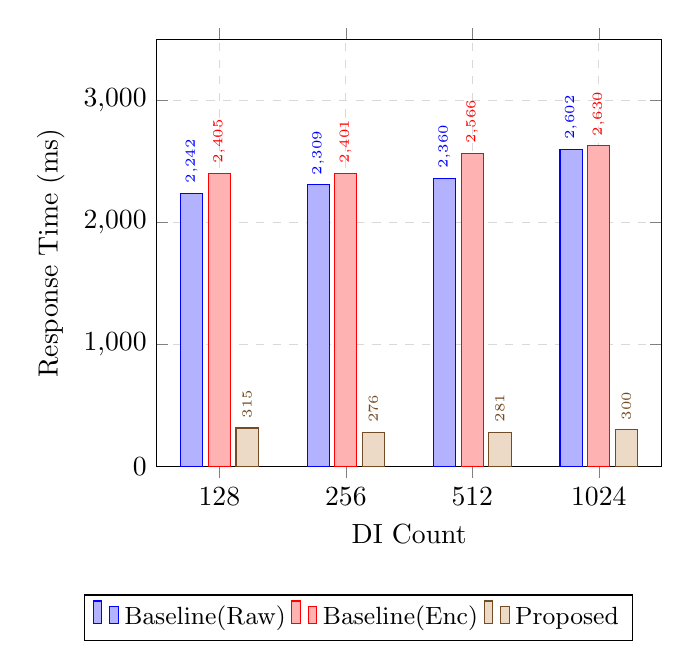
\begin{tikzpicture}
    \begin{axis}[
        ybar,
        enlarge x limits={abs=0.8cm},
        height=7cm,
        width=8cm,
        bar width=8pt,
        ylabel={Response Time (ms)},
        xlabel={DI Count},
        symbolic x coords={128, 256, 512, 1024},
        xtick=data,
        nodes near coords,
        nodes near coords style={rotate=90, anchor=west, font=\tiny, /pgf/number format/fixed},
        ymin=0,
        ymax=3500,
        legend style={at={(0.4,-0.3)}, anchor=north, legend columns=-1, font=\small},
        grid=major,
        grid style={dashed, gray!30},
    ]

    % Baseline (Raw)
    \addplot coordinates {(128, 2242) (256, 2309) (512, 2360) (1024, 2602)};
    
    % Baseline (Encrypted)
    \addplot coordinates {(128, 2405) (256, 2401) (512, 2566) (1024, 2630)};
    
    % Proposed
    \addplot coordinates {(128, 315) (256, 276) (512, 281) (1024, 300)};

    \legend{Baseline(Raw), Baseline(Enc), Proposed}
    \end{axis}
    \end{tikzpicture}
    \caption{average query response time for different DI count(single query, page size 30)}
\end{figure}

DI 수를 1024까지 늘려가며 측정한 응답 시간은 위와 같았다. 실시간 증명 생성이 없는 제안 모델은 모든 환경에서 압도적인 성능 차이(7, 8배)을 보여주었다. 앞서 벤치마크 실험에서 확인한 것 처럼, DI 수 증가에 따른 증명 생성 시간의 증가폭은 미미하였다. 따라서 이 실험에서도 baseline 모델의 전체 응답 시간의 변화는 DI 수의 증가폭에 비해 현저히 작은 것을 볼 수 있다. 또한 암호화 여부가 응답 시간에 미치는 영향은 최소 28ms(1024 DI)에서 최대 206ms(512 DI)에 불과했다. 이는 전체 응답 시간의 최대 0.09\%에 불과하다. 이처럼 데이터의 암호화 여부 역시 전체 응답 시간에서 차지하는 비율은 미미한 것을 볼 수 있다. 결국 응답 시간에 절대적인 영향을 미치는 것은 개별 증명 생성 시간이라는 것을 명백히 알 수 있다.

\begin{figure}[H]
    \centering
    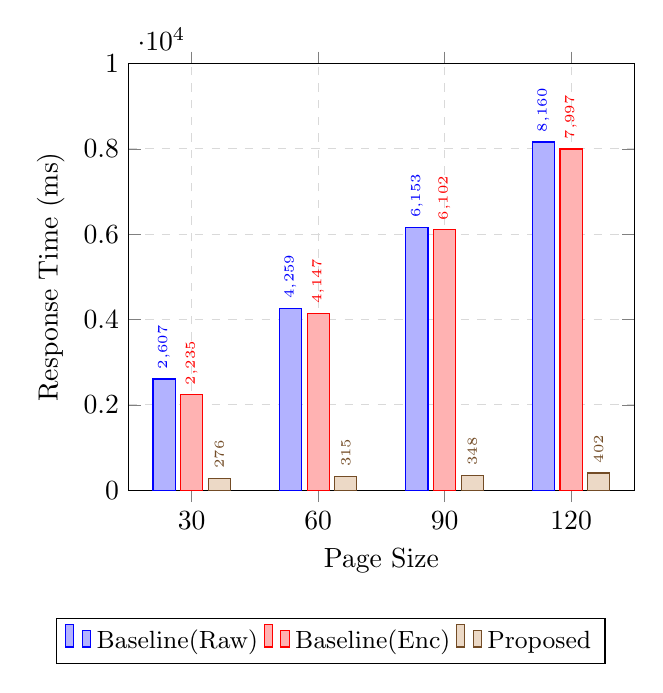
\begin{tikzpicture}
    \begin{axis}[
        ybar,
        enlarge x limits={abs=0.8cm},
        height=7cm,
        width=8cm,
        bar width=8pt,
        ylabel={Response Time (ms)},
        xlabel={Page Size},
        symbolic x coords={30, 60, 90, 120},
        xtick=data,
        nodes near coords,
        nodes near coords style={rotate=90, anchor=west, font=\tiny, /pgf/number format/fixed},
        ymin=0,
        ymax=10000,
        legend style={at={(0.4,-0.3)}, anchor=north, legend columns=-1, font=\small},
        grid=major,
        grid style={dashed, gray!30},
    ]

    % Baseline (Raw)
    \addplot coordinates {(30, 2607) (60, 4259) (90, 6153) (120, 8160)};
    
    % Baseline (Encrypted)
    \addplot coordinates {(30, 2235) (60, 4147) (90, 6102) (120, 7997)};
    
    % Proposed
    \addplot coordinates {(30, 276) (60, 315) (90, 348) (120, 402)};

    \legend{Baseline(Raw), Baseline(Enc), Proposed}
    \end{axis}
    \end{tikzpicture}
    \caption{average query response time for different page size(single query, 128 DI)}
\end{figure}

페이지 크기에 따른 응답 시간의 변화를 보면 이 점을 더욱 극명하게 확인할 수 있다. 페이지 크기를 늘린다는 것은 하나의 쿼리를 처리하는데 그만큼 더 많은 영지식 증명을 처리해야 한다는 의미이다. 위 그래프는 같은 환경에서 페이지 크기를 30에서 120까지 늘렸을 때의 응답 시간의 변화를 나타낸다. 페이지 크기가 커질 수록 baseline 모델은 증명 생성에 대한 부담이 선형적으로 증가하지만, 제안 모델은 그저 데이터베이스 조회 시간만 조금 늘어날 뿐이다. Baseline 모델은 페이지 크기가 30씩 증가할 때 마다 최소 30\%에서 최대 85\%까지도 응답시간이 증가한 반면, 제안 모델은 최소 10\%에서 최대 15\%가 증가하는 수준에 그쳤다. 이처럼 사전 생성된 증명을 채택한 제안 모델은 파라미터의 크기에 관계 없이 안정적인 확장성을 보여주고 있다.

\subsection{위협 모델 시뮬레이션 및 확장 보안에 대한 고찰}

\subsubsection{추론 공격 시뮬레이션 결과}

\begin{figure}[h]
    \centering
    \includegraphics[width=1\linewidth]{figure15-1.png}
    \includegraphics[width=1\linewidth]{figure15-2.png}
    \caption{Simulated adversary view}
\end{figure}

본 시스템의 취약점의 실질적인 위험을 평가하기 위해, 본 연구의 실험 데이터베이스가 모두 유출되었다는 가정하에 공격자 시점에서의 추론 공격(Inference Attack) 시뮬레이션을 수행하였다. 실험에 사용된 OWNERSHIP 테이블을 PROOF와 결합하여 각 DP가 가진 데이터들을 분류, 속성에 따라 각각의 그래프로 시각화 하였다. Figure 14는 특정 개인(DP)으로 부터 알아낼 수 있는 모든 정보를 시각화 한 결과이다. 공격자는 특정 DP가 소유한 모든 데이터의 종류, 수량과 범위의 분포을 알 수 있으며, 이에 기반해 개인에 대한 종합적인 건강 정보를 추론할 수 있다. 그래프에서 나타나듯, 공격자는 개별 튜플의 정확한 평문 수치를 알 수는 없으나, 붉은 선과 푸른 선 사이의 영역에 데이터 원문이 존재한다는 사실은 확인할 수 있다. 본 시스템에서 사용되는 범위 정보는 실제 의학적 참고 수치에 기반하였기 때문에, 이 정도 정보만으로도 해당 개인의 유병 내역(예: 당뇨, 고혈압 등)을 쉽게 예측할 수 있다. 

\bigskip

Figure 14의 실험결과를 해석하면 다음과 같다: 식별자 '0a3f578b-9230-4894-85ea-853b10505bcb'를 가진 개인(DP)은 30개의 속성에 대해 총 1066개의 데이터를 가지고 있었다. 이 중 공복혈당(Fasting Blood Sugar)은 0과 최대치 사이에 37개의 데이터가 분포해 있음을 알 수 있었다. 이 중 당뇨로 판정되는 125 이상의 데이터는 총 14개를 확인하였다. (참고로 해당 실험에 사용된 데이터셋은 난수에 기반해 생성되어 이같은 무작위적인 분포를 보였지만, 실제 데이터의 경우 훨씬 더 일관된 추세를 보일 것으로 예상된다.) 종합하면 공격자는 이 개인이 어떤 시점에 검진을 받았는지, 어떤 검사를 진행했는지, 그리고 데이터의 범위 분포 및 변화의 추이를 파악 할 수 있다. 나아가 이에 기반해 어떤 진단을 받았는지, 특정 시기의 건강 패턴이나 생활 습관이 어떻게 변화했는지 등을 추론해낼 수 있다. 여기에 전문적인 의학적 지식을 동원한다면 다른 속성 정보를 결합해 해당 개인에 대한 더 정확하고 종합적인 건강 정보를 추론해낼 수 있을 것이다.

\subsubsection{위협 완화 전략 및 트레이드오프}
이러한 구조적 위협을 완화하고 시스템을 고도화하기 위해, 본 연구는 다음과 같은 추가적인 보안 전략의 적용을 제안한다.

\bigskip

첫째, 더미 데이터 주입을 통한 교란이다. DI 혹은 DP측에서 최초로 증명을 생성할 때, 실제 데이터와 다른 범위에 속하는 데이터를 생성, 이에 대한 더미 증명을 생성한다. 이처럼 모든 증명에 대해, 수학적으로는 참이지만 실존하지는 않는 거짓 양성(false positive) 증명을 1대 1로 생성하여 SS에 전달한다. 여기서 어느 쪽이 진짜 증명인지는 오직 이를 생성한 DI 혹은 DP만이 알고 있으며, SS 조차도 이를 알 수 없다. 데이터 수요자(DC)는 데이터 구매 결정 후 소유자로부터 데이터 원문을 넘겨받는 시점에서 진짜 증명을 구분할 수 있게 한다. 이 경우 공격자가 소유권 정보를 탈취하여 분석하더라도, 가짜 증명으로 발생한 노이즈로 인해 특정 개인의 병력을 확정적으로 추론하는 것이 불가능해진다. 다만 이러한 구조는 공격자 뿐만 아니라 수요자의 검색 결과에게도 노이즈를 추가하게 되므로 구매 과정에서 이를 효율적으로 필터링 해내는 추가적인 시스템이 요구된다.

\bigskip

둘째, 비공모 다중 서버(Non-colluding Multi-server) 기반의 비밀 분산(Secret Sharing)이다. 검색 서버를 서로 공모하지 않는 두 개 이상의 독립된 서버로 분리하고, OWNERSHIP 테이블의 식별자 정보를 안전한 다자간 컴퓨팅(MPC) 프로토콜을 통해서만 연산되도록 분산 저장하는 방식이다. 이는 현실적으로 적용 가능한 가장 안정적인 방법이며, 더미 데이터 주입과 달리 데이터 수요자 측에 부담을 주지 않는다는 장점이 있다. 공격자는 특정 임계값을 넘는 숫자의 서버를 해킹하지 않는 이상 복호화 키를 복원할 수 없으며, 이를 통해 단일 서버가 장악되더라도 소유권 정보가 복원되지 않는 강력한 기밀성을 확보할 수 있다. 단, 이는 SS 측의 연산 오버헤드를 크게 증가시키는 방법이며, MPC 프로토콜이 검색의 실시간성에 끼치는 영향은 별도의 실험이 필요할 것이다.

\bigskip

결론적으로, 현재 상황에서 본 시스템이 지닌 보안 취약점을 완벽히 보완할 방법은 없어보인다. 어떤 방법을 선택하더라도 사용자 편의성의 희생, 검색의 실시간성의 손실 혹은 연산 비용의 증가는 필수 불가결한 부작용으로 판단된다. 따라서 본 연구는 대규모 데이터 검색의 실시간성과 실용성을 달성하기 위해 OWNERSHIP 테이블 유지라는 전략적 타협을 선택하였다. 향후 위에서 제시한 더미 주입 및 다중 서버 기반의 비밀 분산 기법 등을 발전시킴으로써 부작용은 최소화 하며 최악의 보안 위협까지 완벽히 방어할 수 있는 범용적인 시스템으로 확장할 수 있기를 기대한다.
